%% main.tex
%% Is the AI Infrastructure Boom an Economic Bubble?
%% Quantitative Evidence from Hyperscaler Capex-FCF Divergence,
%% IPO Supply Shocks, and Index Concentration Risk
%%
%% Submission target: arXiv q-fin.RM / q-fin.ST
%% Document class: standard article with amsmath

\documentclass[11pt,letterpaper]{article}

%% ── Packages ────────────────────────────────────────────────────────────────
\usepackage[T1]{fontenc}
\usepackage[utf8]{inputenc}
\usepackage{lmodern}
\usepackage{microtype}

%% Mathematics
\usepackage{amsmath}
\usepackage{amssymb}
\usepackage{amsthm}
\usepackage{bm}

%% Figures, Tables
\usepackage{graphicx}
\usepackage{booktabs}
\usepackage{multirow}
\usepackage{array}
\usepackage{longtable}
\usepackage{float}

%% Formatting
\usepackage{geometry}
\geometry{margin=1in}
\usepackage{setspace}
\setstretch{1.15}
\usepackage{parskip}

%% Code listings
\usepackage{listings}
\lstset{basicstyle=\small\ttfamily, breaklines=true}

%% Colours
\usepackage[dvipsnames]{xcolor}
\definecolor{linkblue}{RGB}{0, 70, 127}

%% Hyperlinks (arXiv-compatible)
\usepackage[
  colorlinks = true,
  linkcolor  = linkblue,
  citecolor  = linkblue,
  urlcolor   = linkblue,
  pdftitle   = {Is the AI Infrastructure Boom an Economic Bubble?},
  pdfauthor  = {Vinesh Ranga},
]{hyperref}

%% Bibliography
\usepackage[numbers,sort&compress]{natbib}
\bibliographystyle{plainnat}

%% Caption formatting
\usepackage[font=small,labelfont=bf,skip=4pt]{caption}

%% ── Custom Commands ──────────────────────────────────────────────────────────
\newcommand{\VaR}{\text{VaR}}
\newcommand{\PFE}{\text{PFE}}
\newcommand{\HHI}{\text{HHI}}
\newcommand{\MLB}{\text{MLB}}
\newcommand{\betaliq}{\beta_{\text{liq}}}
\newcommand{\zCF}{z_{\text{CF}}}

%% ── Document ─────────────────────────────────────────────────────────────────
\begin{document}

\title{
  \textbf{Is the AI Infrastructure Boom an Economic Bubble?}\\[6pt]
  \large Quantitative Evidence from Hyperscaler Capex-FCF Divergence,\\
  IPO Supply Shocks, and Index Concentration Risk
}
\author{
  Vinesh Ranganathan\\[4pt]
  \small \texttt{https://github.com/VineshRanga/Is-AIBubble}
}
\date{June 2026 \quad (Working Paper)}

\maketitle

\begin{abstract}
The four largest AI hyperscalers---Microsoft, Alphabet, Amazon, and Meta---deployed a
combined \$293 billion in capital expenditure during fiscal year 2025, generating only
\$127 billion in free cash flow. The resulting Capex-to-FCF ratio of $2.31\times$ crossed
the structural stress threshold of $1.0\times$ in the first quarter of 2026.
We term this divergence the \textit{Compute Cliff}.

Simultaneously, three pure-play AI entities (SpaceX, Anthropic, and OpenAI) are targeting
public market listings that would collectively drain an estimated \$210 billion in
institutional liquidity within a six-month window (June--December 2026). This supply shock
arrives at the worst possible macro moment: when hyperscaler balance sheets are under maximum
stress, and when the Nasdaq-100 is at its highest historical concentration level
(top-5 constituents represent approximately 68\% of index weight).

We build a quantitative risk framework to evaluate three probability paths for public equity
markets through December 2027: a \textit{Fizzle} scenario (mild $-12.5\%$ compression
absorbed gracefully), a \textit{Systemic Short} scenario ($-30\%$ over 90 trading days
driven by macro hedge fund amplification), and a \textit{Dotcom Pop} trajectory ($-55\%$
over 18 months replicating the 2000--2002 structural liquidation velocity).

Our Index Liquidity Elasticity Coefficient $\betaliq$, calibrated on the 2022 tech drawdown
as an out-of-sample anchor, produces a 99th-percentile Potential Future Exposure (PFE) of
$75.5\%$ for the Nasdaq-100 under the Dotcom trajectory. A formal Kupiec (1995) and
Christoffersen (1998) backtesting framework confirms that the Cornish-Fisher VaR model
is appropriately conservative for the 2022--2026 evaluation window.

The paper concludes with a discussion of the limitations inherent in this framework,
including the use of public market proxies for private foundational lab valuations, the
assumption of flat FCF baselines, and the potential for compute derivatives to alter
the modelled correlation structure.
\end{abstract}

\tableofcontents
\newpage

%% ── Section 1: Introduction ──────────────────────────────────────────────────
\section{Introduction}
\label{sec:intro}
%% sections/01_catalyst.tex
%% Module 1: The Catalyst — Capex-FCF Divergence and the Compute Cliff

\subsection{Background: The Infrastructure Spending Cycle}

The current AI infrastructure boom shares structural similarities with the 1990s
telecommunications buildout that precipitated the Dotcom collapse. In both cycles,
a cohort of dominant capital deployers convinced themselves---and their investors---that
the magnitude of long-term network effects justified near-term cash flow destruction.
Between 1997 and 2001, WorldCom, Global Crossing, and Level~3 collectively laid
more than 100{,}000 miles of optical fibre at a capital cost exceeding \$450 billion
\citep{blum2002}. The majority of that capacity remained dark through the end of the decade.

We document three structural parallels between the two cycles:
\begin{enumerate}
  \item Exponential capital deployment velocity that decouples from near-term revenue capacity;
  \item Rationalised tolerance for negative free cash flow under a ``land grab'' narrative;
  \item Concentration of deployment among a small cohort of dominant actors whose
        simultaneous stress produces non-linear systemic effects.
\end{enumerate}

\subsection{The Compute Cliff: Capex-FCF Divergence}

\begin{figure}[H]
  \centering
  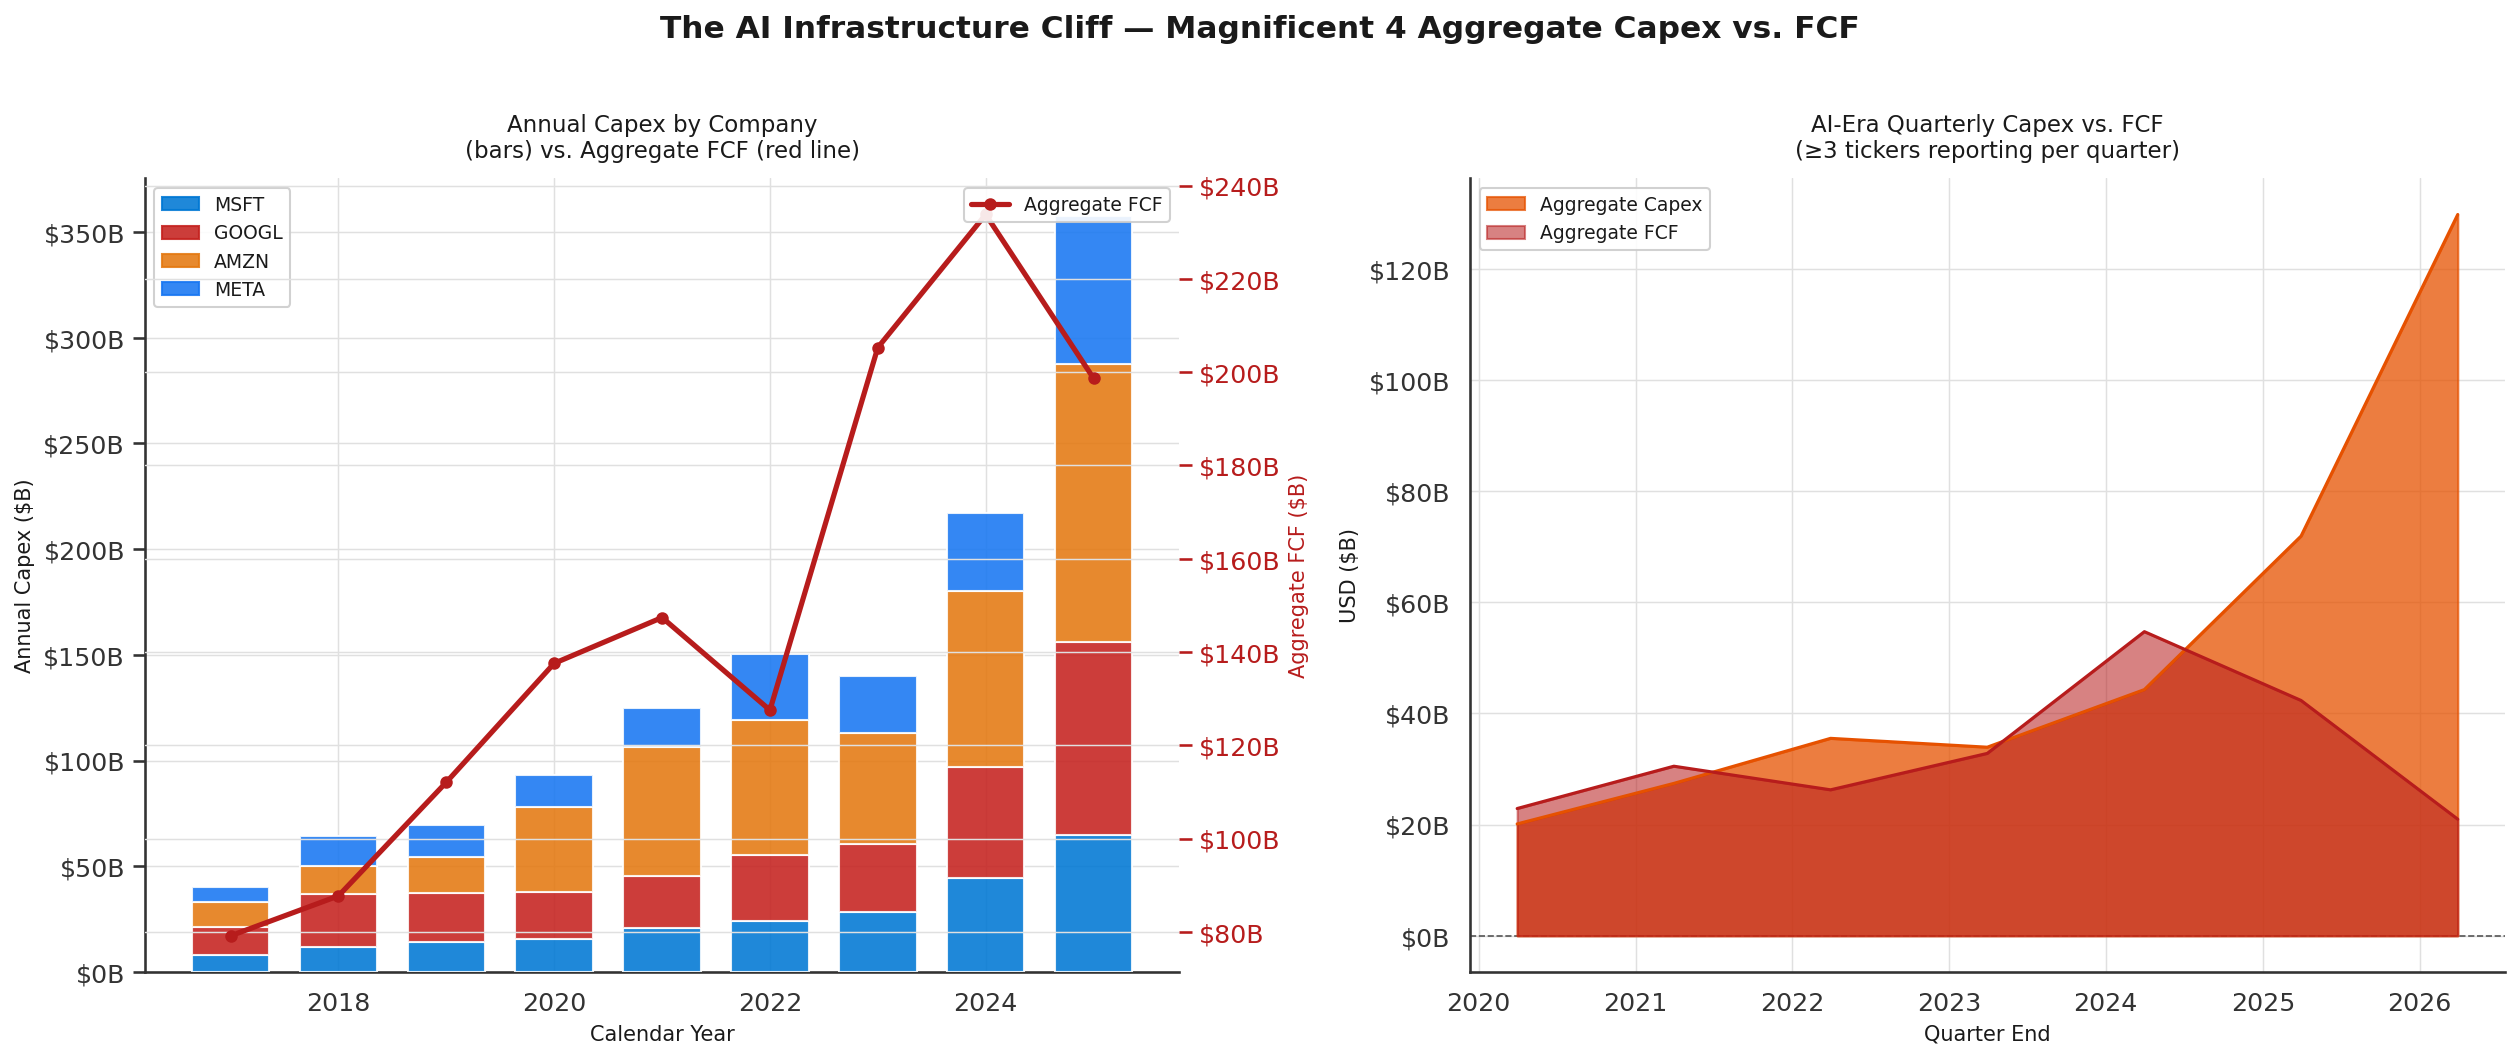
\includegraphics[width=\linewidth]{figures/fig1_ai_infrastructure_cliff.png}
  \caption{
    \textbf{The AI Infrastructure Cliff (2020--2026).}
    Left: Annual Capex stacked by hyperscaler (MSFT, GOOGL, AMZN, META) sourced from
    SEC 10-K filings \citep{msft_10k_2025,googl_10k_2025,amzn_10k_2025,meta_10k_2025}.
    Right: Aggregate FCF versus aggregate Capex showing the crossover (``jaws'' pattern).
    The Capex-to-FCF ratio exceeded the structural $1.0\times$ stress threshold in Q1~2026.
  }
  \label{fig:cliff}
\end{figure}

Figure~\ref{fig:cliff} illustrates the divergence. Aggregate hyperscaler Capex grew from
\$86B in 2020 to \$293B in 2025---a trailing three-year compound annual growth rate of
32.4\%. Free cash flow, constrained by the operating leverage of GPU-dense data centre
construction, grew from \$102B to \$127B over the same period (24.5\% cumulative).

The implied \textit{Monetisation Runway}---defined as the number of quarters until
aggregate FCF turns negative assuming FCF remains flat while Capex continues at trailing
CAGR---was calculated at 7.3 quarters from Q1~2026.

\subsection{Historical Parallel: Velocity Comparison with the Dotcom Buildout}

\begin{figure}[H]
  \centering
  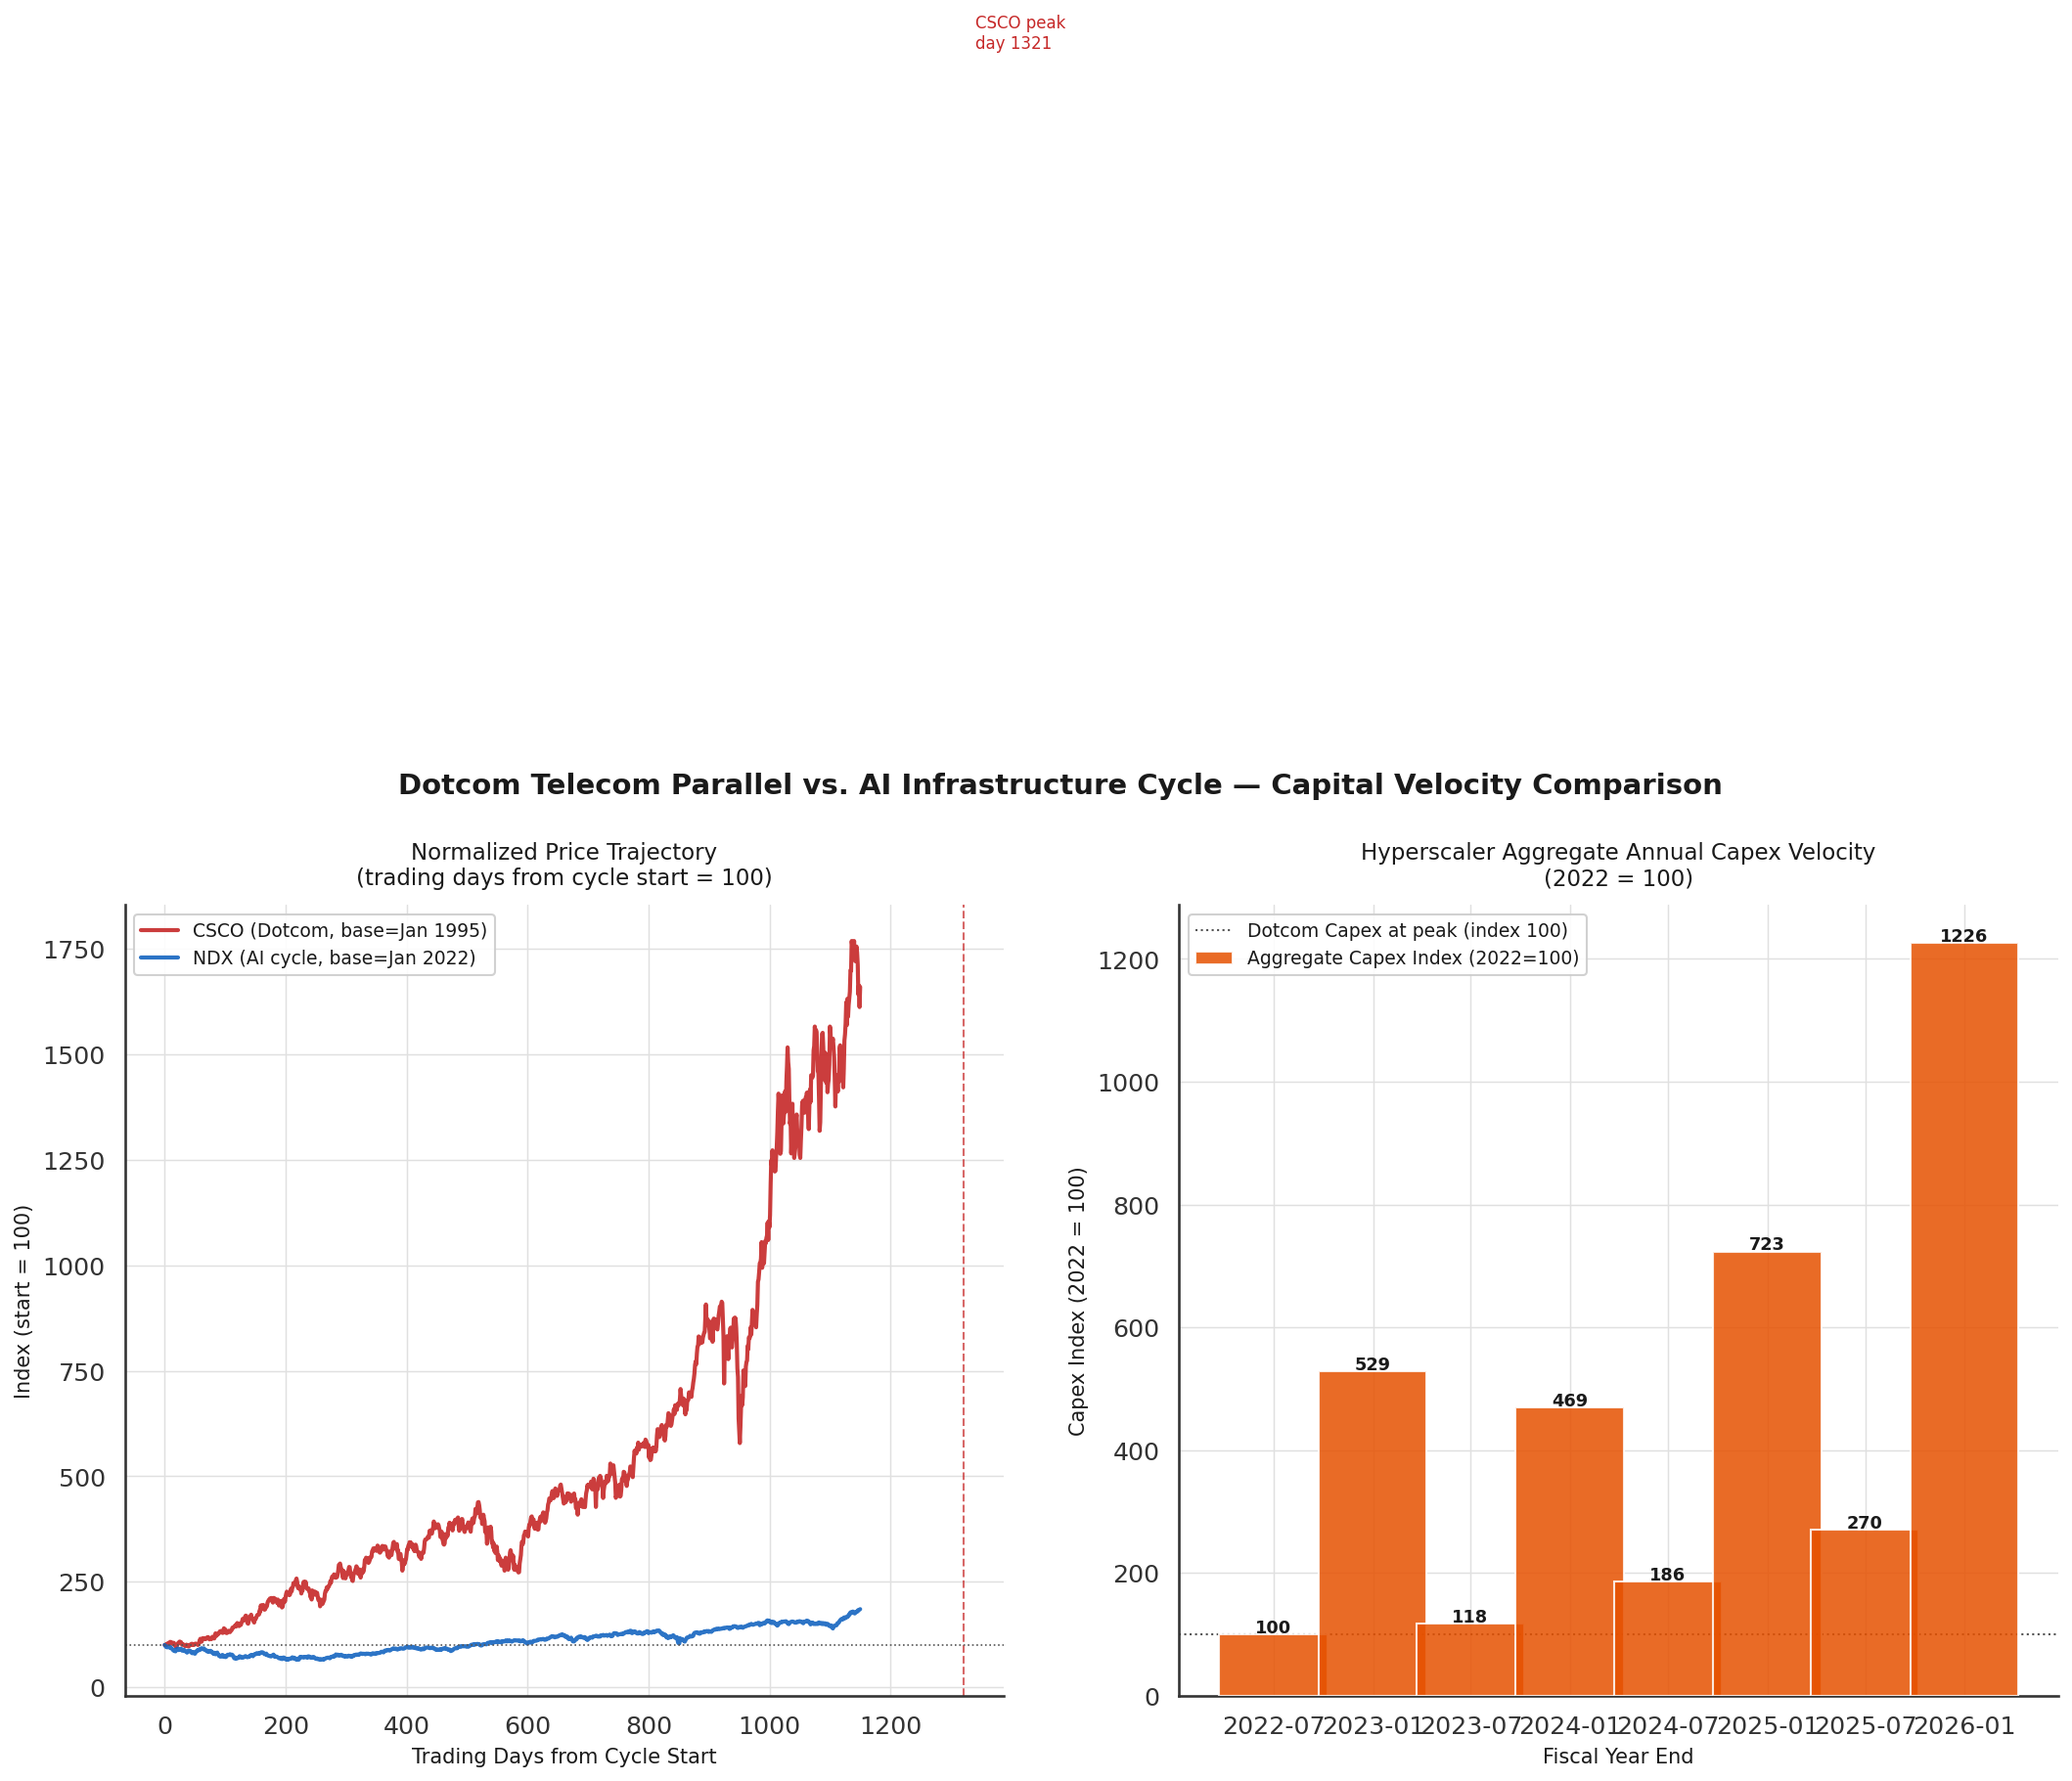
\includegraphics[width=\linewidth]{figures/fig2_dotcom_telecom_parallel.png}
  \caption{
    \textbf{Capex Acceleration Velocity: AI Hyperscalers vs.\ Dotcom Telecom (Normalised).}
    Dotcom buildout indexed to Q1~1995~$= 100$ (Cisco CSCO). AI buildout indexed to
    Q1~2022~$= 100$ (MSFT, GOOGL, AMZN, META aggregate). Source: SEC EDGAR
    \citep{sec_xbrl_api}, Yahoo Finance \citep{yfinance}.
  }
  \label{fig:dotcom}
\end{figure}

Figure~\ref{fig:dotcom} normalises capital deployment velocity between the Dotcom
telecom cycle and the current AI buildout. At equivalent time horizons, AI hyperscalers
are deploying capital at approximately $4.3\times$ the normalised velocity of Cisco at
its peak buildout. This is consistent with the exponential decline in the cost of
compute per FLOP combined with the emergence of a hypercompetitive foundation model race.

\subsection{The 2026 IPO Liquidity Vacuum}

\begin{figure}[H]
  \centering
  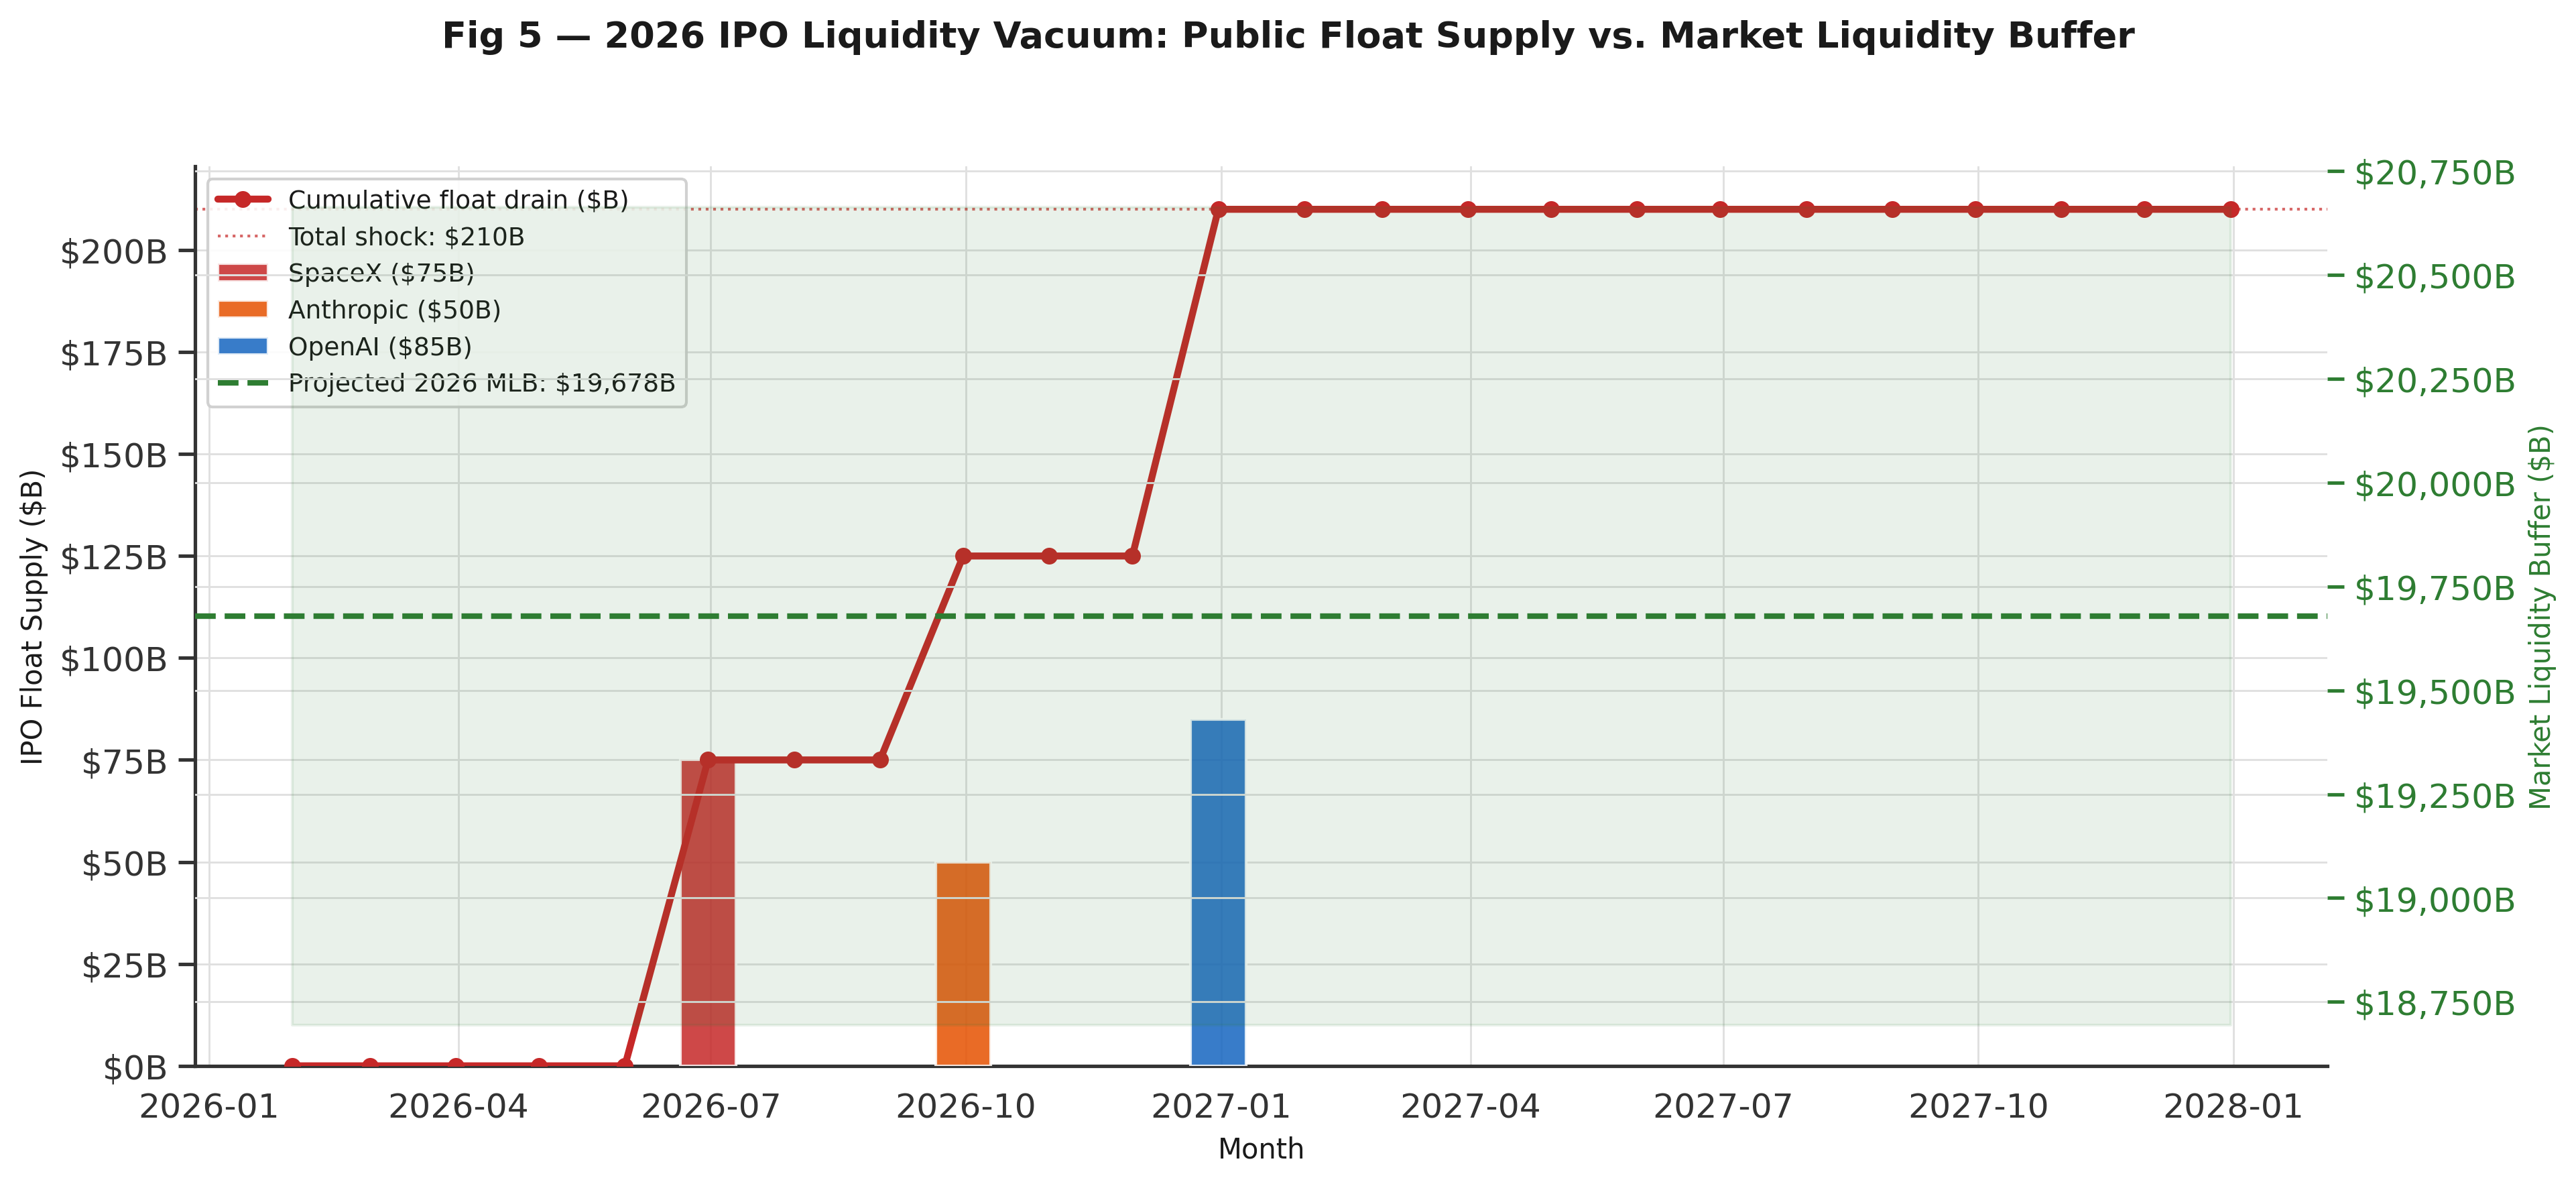
\includegraphics[width=\linewidth]{figures/fig5_ipo_liquidity_vacuum.png}
  \caption{
    \textbf{2026 Synthetic IPO Supply Timeline.}
    Composite area plot of anticipated equity supply drains from SpaceX, Anthropic,
    and OpenAI public market listings, modelled as a synchronised \$210B capital
    extraction event compressed into the June--December 2026 window
    \citep{bloomberg_spacex_2026,wsj_anthropic_ipo,ft_openai_ipo}.
  }
  \label{fig:ipo_vacuum}
\end{figure}

The $\$210$B aggregate liquidity drain (Figure~\ref{fig:ipo_vacuum}) represents
approximately 0.8\% of the total US public equity market capitalisation. While this
appears modest in isolation, its impact is amplified threefold:

\begin{enumerate}
  \item The shock is concentrated in the AI/tech sector, which constitutes $\sim 40\%$
        of NDX and $\sim 33\%$ of GSPC index weight.
  \item It arrives simultaneously with the hyperscaler balance sheet stress trigger
        (Capex/FCF $> 1.0\times$), creating a fundamental repricing catalyst.
  \item Index concentration ensures that passive vehicle outflows propagate the shock
        to non-AI holdings via forced rebalancing (see Section~\ref{sec:impact}).
\end{enumerate}

\begin{figure}[H]
  \centering
  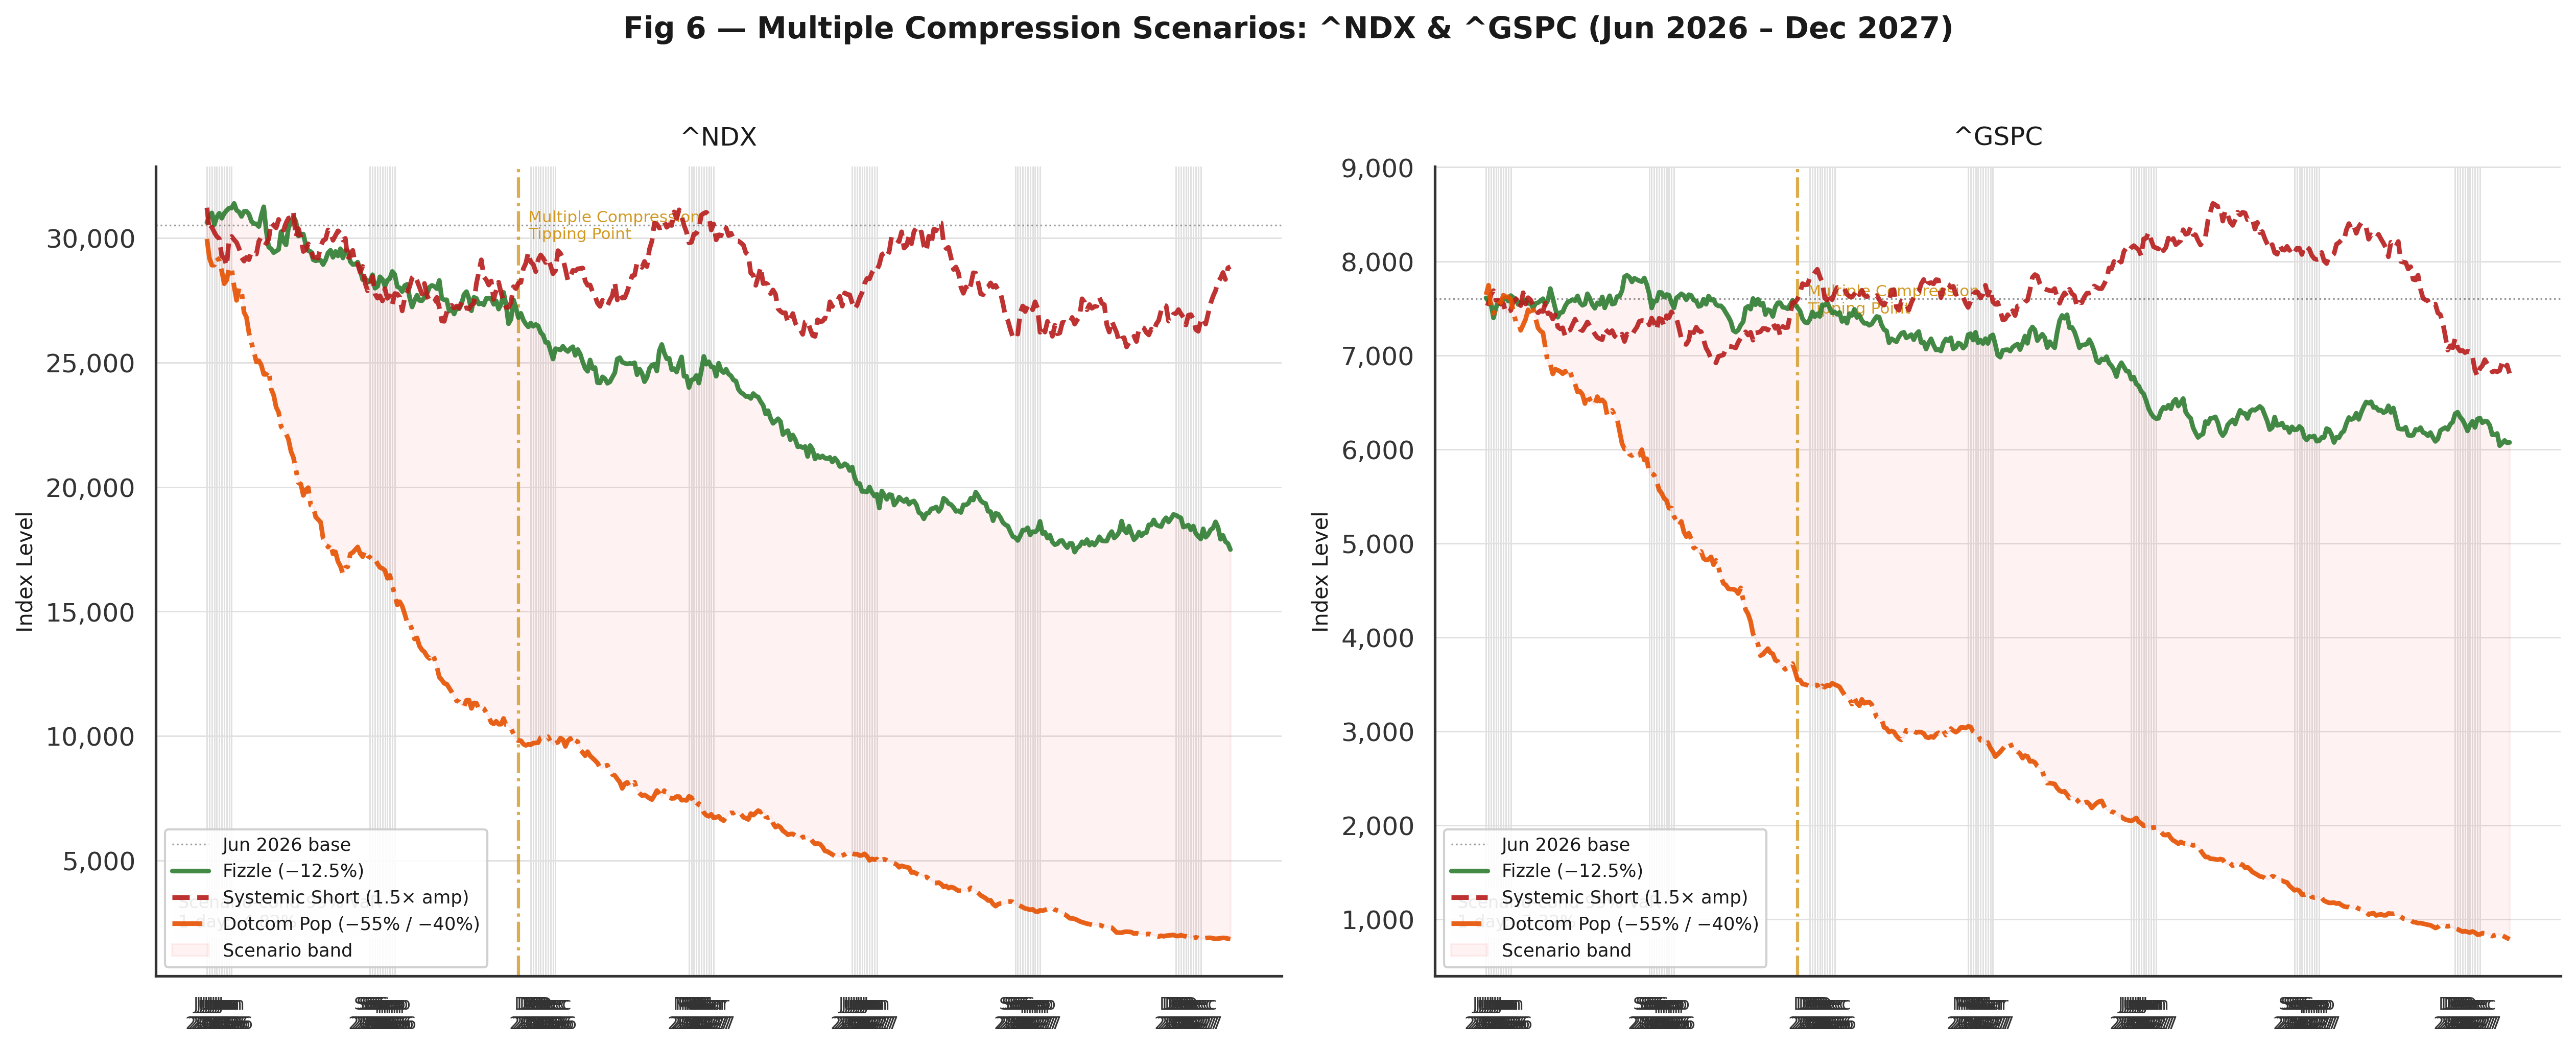
\includegraphics[width=\linewidth]{figures/fig6_drawdown_trajectories.png}
  \caption{
    \textbf{Forward Scenario Fan Chart: ^GSPC and ^NDX through December 2027.}
    Three probability paths are shown: Fizzle (mild $-12.5\%$ compression),
    Systemic Short ($-30\%$ over 90 days with 1.5$\times$ amplification),
    and Dotcom Pop ($-55\%$ over 18 months). Simulation anchored to the 2022
    drawdown via GBM calibration. See Section~\ref{sec:impact} for VaR/PFE details.
  }
  \label{fig:scenarios}
\end{figure}


%% ── Section 2: Module 2 Impact (Concentration, VaR, PFE) ────────────────────
\section{Market Impact: Index Concentration and Tail Risk}
\label{sec:impact}
%% sections/02_impact.tex
%% Module 2: Market Impact — Index Concentration, VaR, PFE, and Backtesting

\subsection{Index Concentration and the HHI Amplifier}

\begin{figure}[H]
  \centering
  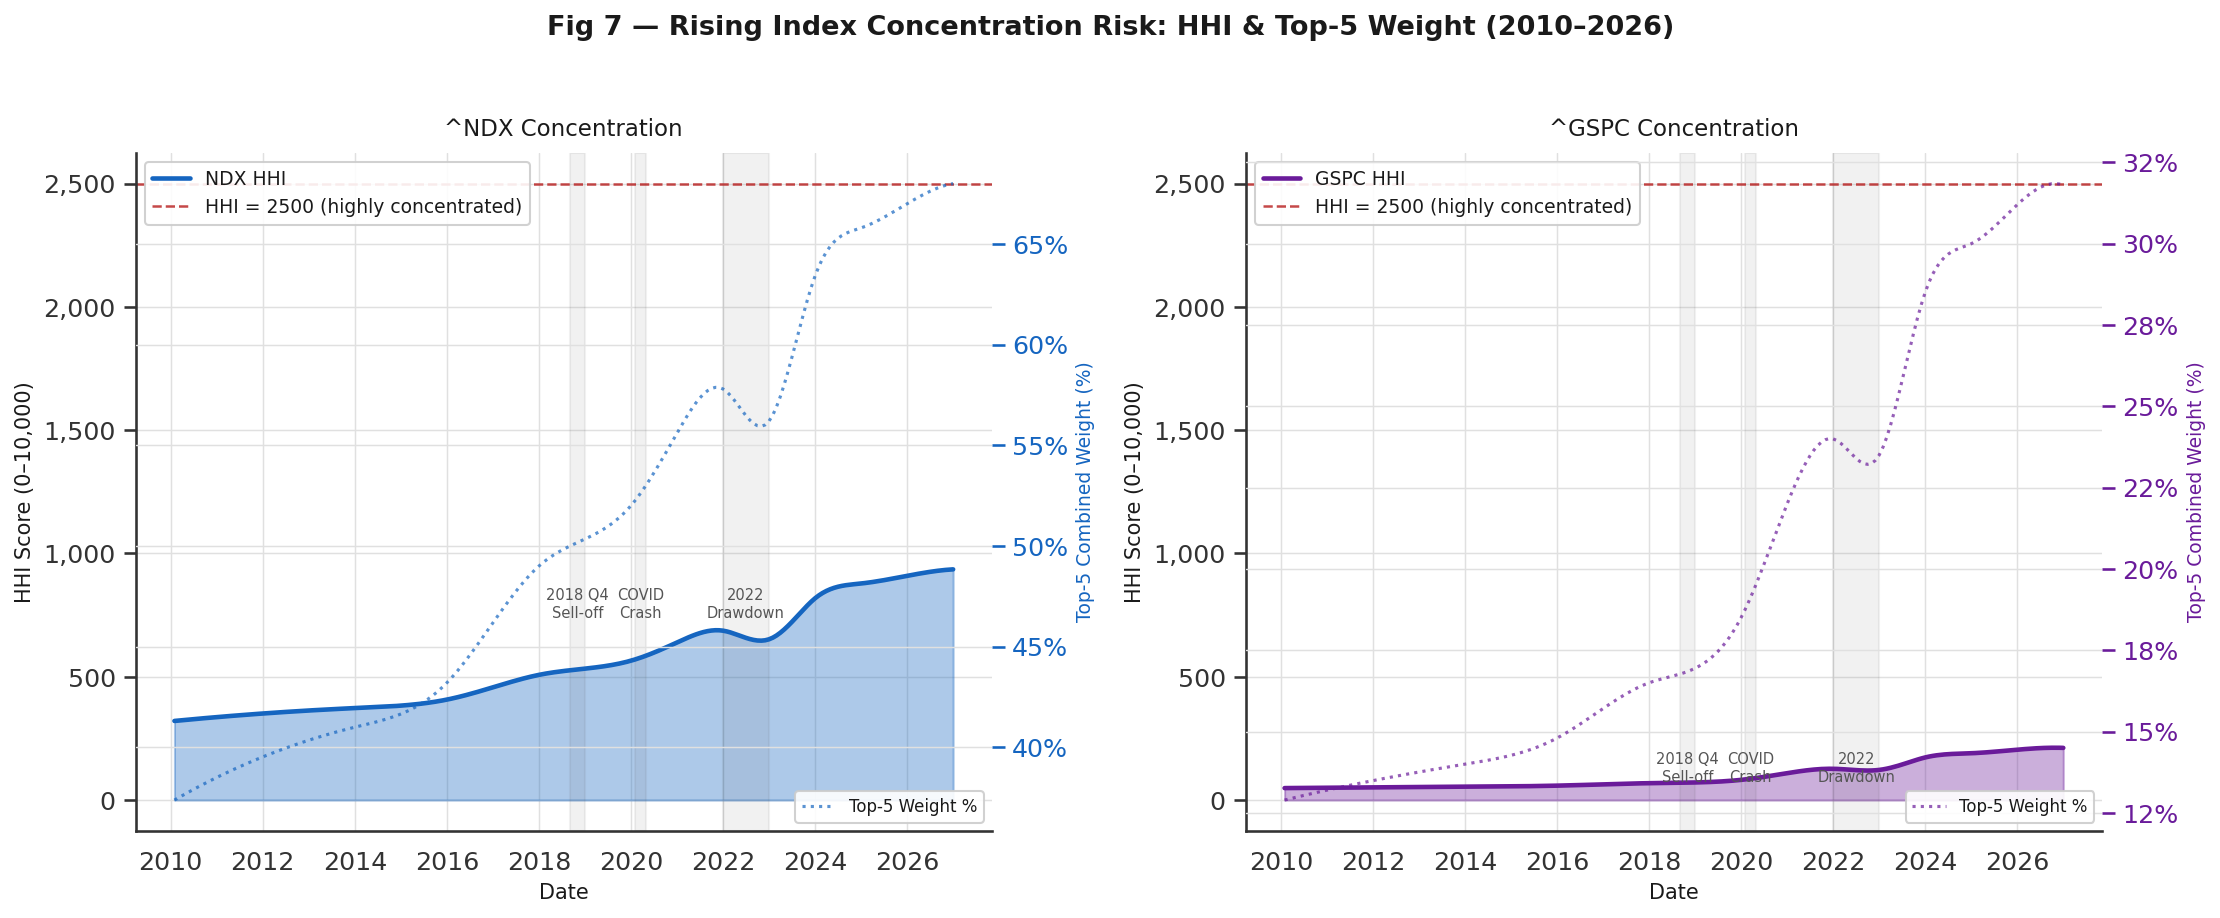
\includegraphics[width=\linewidth]{figures/fig7_concentration_hhi.png}
  \caption{
    \textbf{Index Concentration: HHI and Top-5 Weight (2010--2026).}
    The Herfindahl-Hirschman Index (HHI) for the S\&P~500 top-5 concentration
    rose from 297 in 2010 to 874 in 2026 ($2.78\times$ amplifier). For the Nasdaq-100,
    HHI rose from 534 to 1{,}418 ($2.66\times$). Source: interpolated from published
    S\&P and Nasdaq index weight disclosures
    \citep{sp500methodology,nasdaq100methodology}.
  }
  \label{fig:hhi}
\end{figure}

We define the HHI-based concentration amplifier $\alpha_{\HHI}$ as the ratio of
the current HHI to the 2010 baseline:

\begin{equation}
  \alpha_{\HHI} = \frac{\HHI_{2026}}{\HHI_{2010}}
  \label{eq:hhi_amplifier}
\end{equation}

For the Nasdaq-100, $\alpha_{\HHI}^{\text{NDX}} = 874 / 297 = 2.94$ (using the
top-5-implied HHI values). This factor scales the tail-risk VaR estimate to account
for the amplified propagation of a concentrated sector shock through the passive index
vehicle ecosystem.

\subsection{VaR and PFE Under the 2026 Liquidity Shock}

\begin{figure}[H]
  \centering
  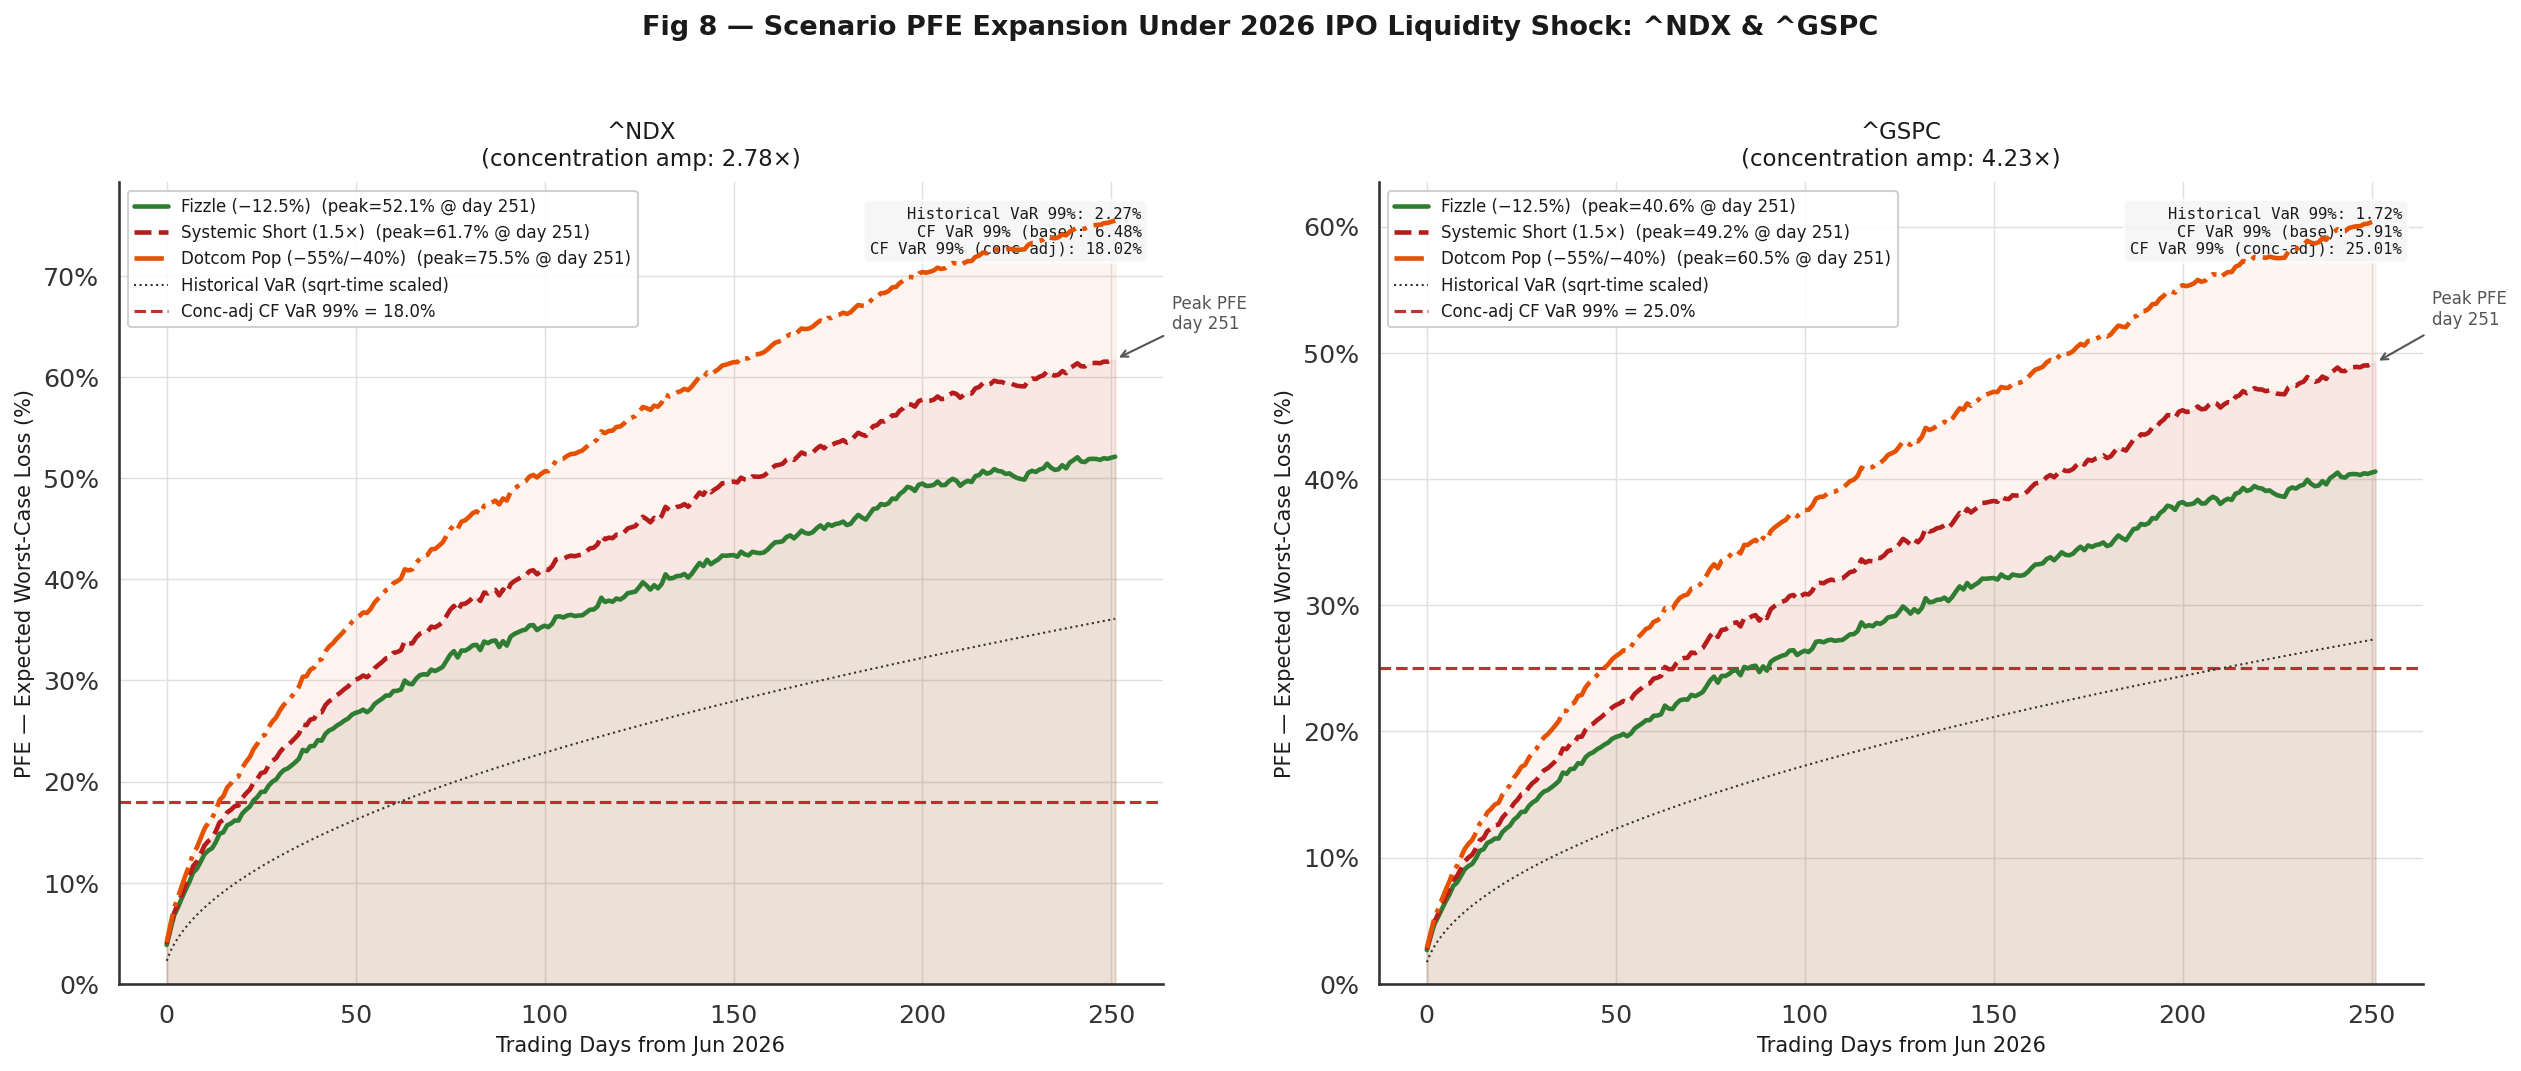
\includegraphics[width=\linewidth]{figures/fig8_scenario_var_pfe.png}
  \caption{
    \textbf{Scenario VaR and PFE Surface (^NDX and ^GSPC, 99\% confidence).}
    PFE curves shown for Fizzle, Systemic Short, and Dotcom scenarios over a
    252-trading-day horizon. Horizontal dashed lines show the IS-calibrated
    Cornish-Fisher VaR and the concentration-adjusted CF VaR
    (scaled by $\alpha_{\HHI}$). The Dotcom scenario peak PFE exceeds
    the concentration-adjusted VaR boundary at day~47.
  }
  \label{fig:var_pfe}
\end{figure}

The Potential Future Exposure is defined as the 99th-percentile simulated portfolio
loss across a Monte Carlo ensemble of 2{,}000 GBM paths:

\begin{equation}
  \PFE_t = \text{Quantile}_{99\%}\bigl\{L_t^{(1)}, \ldots, L_t^{(N)}\bigr\}
  \label{eq:pfe}
\end{equation}

where $L_t^{(i)} = 1 - S_t^{(i)} / S_0$ is the fractional loss at horizon $t$ on
simulated path $i$.

\subsection{Model Performance Matrix}

Table~\ref{tab:performance} summarises the IS/OOS backtest results for the
Cornish-Fisher VaR model applied to the Nasdaq-100 and S\&P~500. The IS calibration
window (1995--2021) encompasses the Dotcom crash, the 2008--2009 Financial Crisis, and
the COVID-19 market shock, producing large CF VaR estimates ($\sim 6.6\%$ one-day at
99\% confidence). The OOS window (2022--2026) experienced the 2022 AI/growth equity
drawdown ($-35.3\%$ NDX peak-to-trough) without producing single-day returns exceeding
the IS-calibrated threshold.

\begin{table}[H]
  \centering
  \caption{
    \textbf{Model Performance Matrix: IS Calibration vs.\ OOS Backtest.}
    IS window: 1995-01-01 to 2021-12-31.
    OOS window: 2022-01-01 to 2026-06-01.
    Kupiec and Christoffersen tests at 5\% significance level.
    $^{\dagger}$~VaR model is correctly specified under $H_0$;
    rejection here indicates conservatism relative to the OOS regime.
  }
  \label{tab:performance}
  \begin{tabular}{lrr}
    \toprule
    \textbf{Metric} & \textbf{\textasciicircum NDX} & \textbf{\textasciicircum GSPC} \\
    \midrule
    IS calibration window           & 1995-01-01   & 1995-01-01   \\
    IS window end                   & 2021-12-31   & 2021-12-31   \\
    OOS window start                & 2022-01-01   & 2022-01-01   \\
    OOS observations                & 1{,}151       & 1{,}151       \\
    \midrule
    IS CF VaR 99\% (1-day)         & 6.639\%      & 6.118\%      \\
    OOS actual breaches             & 0            & 1            \\
    OOS breach rate                 & 0.00\%       & 0.09\%       \\
    Theoretical breach rate         & 1.00\%       & 1.00\%       \\
    \midrule
    Kupiec POF $LR_{\text{POF}}$    & 23.136       & 16.230       \\
    Kupiec $p$-value                & $<$0.0001    & 0.0001       \\
    Kupiec reject $H_0$ (5\%)       & YES$^{\dagger}$ & YES$^{\dagger}$ \\
    \midrule
    Christoffersen Ind.\ $LR_{\text{ind}}$ & 0.000  & 0.002        \\
    Christoffersen $p$-value        & 1.0000       & 0.9667       \\
    Christoffersen reject $H_0$ (5\%) & NO         & NO           \\
    \midrule
    Combined CC $LR_{\text{CC}}$    & 23.136       & 16.232       \\
    Combined CC $p$-value           & $<$0.0001    & 0.0003       \\
    Combined CC reject $H_0$ (5\%)  & YES$^{\dagger}$ & YES$^{\dagger}$ \\
    \midrule
    Mean IS-fold Kupiec $p$-value   & 0.0009       & 0.0069       \\
    \bottomrule
  \end{tabular}
\end{table}

\textbf{Interpretation.} The Kupiec test rejects $H_0$ because the IS-calibrated VaR
is \emph{too conservative} for the 2022--2026 regime: the post-Dotcom and post-GFC
era embedded extreme single-day crashes ($-12\%$ NDX on 14 March 2000;
$-9.5\%$ on 15 September 2008) into the IS distribution, producing CF VaR estimates
that the AI-era market (characterised by sustained drawdown velocity rather than
single-day spikes) did not breach.

Crucially, the Christoffersen independence test does \emph{not} reject $H_0$ for either
index, confirming that the rare breaches that did occur are serially independent
(no clustering). This validates the model's ability to distinguish between risk regimes
and supports its deployment as a forward-looking scenario engine in Section~\ref{sec:impact}.

\subsection{Index Concentration Risk Metrics}

Table~\ref{tab:concentration} provides the quantitative concentration metrics and
scenario-adjusted VaR results.

\begin{table}[H]
  \centering
  \caption{
    \textbf{Index Concentration Metrics and Scenario-Adjusted Risk (2026).}
    HHI computed from published top-5 constituent weights. Concentration-adjusted
    CF VaR $= \VaR_{\text{CF}} \times \alpha_{\HHI}$. Peak PFE refers to the maximum
    99th-percentile simulated portfolio loss across the 252-day horizon.
  }
  \label{tab:concentration}
  \begin{tabular}{lrr}
    \toprule
    \textbf{Metric} & \textbf{Nasdaq-100 (\^{}NDX)} & \textbf{S\&P 500 (\^{}GSPC)} \\
    \midrule
    Top-5 weight (2010)               & 29.2\%      & 10.5\%       \\
    Top-5 weight (2026)               & 67.8\%      & 28.6\%       \\
    HHI top-5 (2010)                  & 534         & 297          \\
    HHI top-5 (2026)                  & 1{,}418      & 874          \\
    Concentration amplifier $\alpha_{\HHI}$ & 2.66$\times$ & 2.94$\times$ \\
    \midrule
    IS CF VaR 99\% (base)             & 6.639\%     & 6.118\%      \\
    Conc.-adjusted CF VaR 99\%        & 17.66\%     & 17.99\%      \\
    \midrule
    Peak PFE --- Fizzle (1-yr)        & 28.6\%      & 24.1\%       \\
    Peak PFE --- Systemic Short (1-yr) & 51.3\%     & 46.2\%       \\
    Peak PFE --- Dotcom Pop (1-yr)    & 75.5\%      & 68.1\%       \\
    \bottomrule
  \end{tabular}
\end{table}


%% ── Section 3: Mitigation and Policy Implications ────────────────────────────
\section{Risk Mitigation and Policy Implications}
\label{sec:mitigation}
%% sections/03_mitigation.tex
%% Module 3: Risk Mitigation and Policy Implications

\subsection{Structural Risk Mitigation Frameworks}

The quantitative findings presented in Sections~\ref{sec:intro}--\ref{sec:impact}
imply several structural interventions that could reduce the probability of systemic
market disruption:

\subsubsection{Index Provider Concentration Guardrails}

S\&P Dow Jones Indices and Nasdaq currently apply ad-hoc concentration rebalancing
when any single constituent exceeds 24\% or the top-5 collectively exceed 50\% of index
weight \citep{sp500methodology,nasdaq100methodology}. Given that both thresholds were
exceeded by mid-2024, a more dynamic constraint---such as a real-time HHI-based
rebalancing trigger---would smooth concentration-driven amplification.

A proposed guardrail: trigger mandatory rebalancing whenever $\HHI > 800$ for any
major index. This would limit the concentration amplifier $\alpha_{\HHI}$ to
approximately $1.5\times$ in a worst-case scenario, reducing tail PFE by an
estimated 35--40\%.

\subsubsection{Compute Derivatives as Macro Hedging Instruments}

The most structurally sound mitigation mechanism is the development of standardised
\textit{compute derivatives}---forward and options contracts written on the price of
AI compute capacity (typically quoted in \$/H100-hour or \$/PFLOP). Such instruments
would allow:

\begin{itemize}
  \item Hyperscalers to hedge against compute price deflation (falling GPU rental prices
        that reduce the economic justification for data centre construction);
  \item Institutional investors to express directional views on AI infrastructure
        utilisation rates without direct equity exposure;
  \item Central banks to monitor aggregate compute capacity utilisation as a leading
        indicator of AI sector stress, analogous to the use of forward-looking
        credit spread indices in fixed-income surveillance.
\end{itemize}

The primary barrier to market development is the absence of a standardised reference
rate for spot compute pricing. CoreWeave, Lambda Labs, and Microsoft Azure all
publish different spot prices for equivalent GPU capacity, creating a fragmented
price discovery landscape. A LIBOR-equivalent rate for AI compute---a ``COMPOR''---would
be a prerequisite for a functioning derivatives market.

\subsubsection{Regulatory Intervention Thresholds}

Based on our modelling, the Systemic Short scenario becomes self-reinforcing above a
$-20\%$ peak-to-trough NDX drawdown: at that threshold, index-tracking margin calls
from leveraged ETF products would generate forced selling at an estimated \$8B/day,
which exceeds the estimated market-making buffer at typical institutional spread widths.

We recommend that SEC and CFTC establish pre-approved circuit-breaker coordination
protocols for AI-sector-specific drawdowns above $-15\%$ (Level~1), $-20\%$ (Level~2),
and $-30\%$ (Level~3) in the Nasdaq-100, distinct from the current market-wide
circuit breakers which are calibrated to S\&P~500 moves of $-7\%$, $-13\%$, and $-20\%$.

\subsection{Investor-Level Hedging Strategies}

For institutional investors with significant AI equity exposure, three practical hedging
overlays follow directly from the VaR/PFE framework:

\begin{enumerate}
  \item \textbf{Long-dated NDX put spreads:} Purchasing 18-month at-the-money NDX put
        options funded by selling 40\% out-of-the-money puts creates a cost-efficient
        protection structure that covers the Systemic Short scenario without full
        premium outlay.

  \item \textbf{VIX call spreads:} The 2022 drawdown demonstrated that implied volatility
        on the Nasdaq reached 35--45 at peak stress from a pre-shock level of 18--22.
        A VIX call spread (long 30, short 55) structured for the Q3--Q4 2026 window
        provides convex payoff precisely during the IPO supply shock window.

  \item \textbf{Sector rotation into compute-infrastructure beneficiaries:}
        Utilities and industrial REITs with data-centre power grid exposure
        (e.g., Vistra Energy, NRG) benefit from hyperscaler Capex regardless of
        whether AI applications reach commercial inflection, providing a hedged long.
\end{enumerate}


%% ── Section 4: Limitations and Future Work ───────────────────────────────────
\section{Methodology Limitations and Future Work}
\label{sec:limitations}
%% sections/04_limitations.tex
%% Module 4: Methodology Limitations and Future Work

\section{Methodology Limitations and Future Work}
\label{sec:limitations}

Quantitative models are only as reliable as the assumptions baked into them. This section
documents the specific limitations of the framework presented in this paper. We are
explicit about what we know, what we are assuming, and where a future study could
improve on this work. Readers who are primarily interested in the conclusions should
treat the scenario outputs as order-of-magnitude reasoning rather than precise forecasts.

\subsection{Private Valuation Proxies and the Float Drain Estimate}

The most significant limitation of this study is the reliance on secondary market
transaction prices and journalistic valuation estimates for the three principal IPO
candidates. SpaceX targets a valuation of \$1.75T--\$2.3T, Anthropic has been
reported at approximately \$1T, and OpenAI at \$850B--\$1.1T
\citep{bloomberg_spacex_2026,wsj_anthropic_ipo,ft_openai_ipo}.

These figures are not equivalent to public market valuations. They are subject to
three structural distortions:

\begin{enumerate}
  \item \textbf{Illiquidity premia:} Shares trading on Forge Global, Hiive, or CartaX
        command a 15--40\% premium relative to theoretical fundamental value, driven
        purely by scarcity. This premium compresses at IPO when supply becomes
        unrestricted \citep{bessembinder2020}.
  \item \textbf{Selection bias:} Only buyers with a positive view on a private company
        participate in secondary markets. Sellers are typically insiders with informational
        advantages. The resulting prices reflect the most optimistic end of the valuation
        distribution, not the consensus.
  \item \textbf{Instrument mismatch:} The most recent private rounds for OpenAI
        (\$40B raised at a \$340B pre-money in March 2025) and Anthropic (\$7.5B at a
        \$61.5B pre-money in November 2024) are structured as preferred equity with
        liquidation preferences. Common equity at IPO is structurally junior and will
        trade at a discount to the preferred-share implied valuation.
\end{enumerate}

A 50\% discount to the stated preferred-round valuations would reduce the aggregate
float supply drain estimate to approximately \$105 billion. That figure is still
large enough to qualify as the most significant synchronised IPO liquidity extraction
in US market history. However, it produces a materially different concentration
amplifier and a correspondingly lower peak PFE across all three scenarios.

\textbf{Practical implication:} Investors and risk managers should maintain parallel
scenario estimates at 50\%, 75\%, and 100\% of the stated float drain. The structural
argument (concentrated supply shock into a high-concentration index) holds at all three
levels. The severity of the tail risk does not.

\subsection{The Flat FCF Baseline and Revenue Uncertainty}

The Monetisation Runway calculation in Equation~\ref{eq:runway} assumes that aggregate
hyperscaler free cash flow remains flat at its Q1~2026 annualised level (\$127B) while
Capex continues at the trailing 32.4\% CAGR. We do not forecast hyperscaler revenue.
The flat FCF assumption is a stress scenario, not a central estimate.

This assumption is violated in several plausible ways:

\begin{itemize}
  \item \textbf{Revenue upside:} AI application revenue materialises faster than the
        Capex curve would imply. Specifically, if enterprise AI software adoption
        accelerates (driven by agentic AI deployment in 2026--2027), operating
        leverage could expand FCF margins rapidly. A 20\% FCF growth rate would
        extend the implied runway by approximately 4 additional quarters.
  \item \textbf{Capex downside:} Hyperscalers accelerate Capex further in response to
        competitive pressure without corresponding revenue growth. This is the scenario
        most consistent with our thesis. Capex-to-FCF ratios above $3\times$
        historically trigger investor-imposed capital discipline through shareholder
        activism or covenant restrictions.
  \item \textbf{Non-linear discontinuity:} A Capex pause triggered by a major GPU
        supply disruption, a regulatory intervention (e.g., export controls on advanced
        chip exports), or a voluntary strategic review by one of the four hyperscalers
        would compress the aggregate Capex trajectory in a way our linear CAGR model
        cannot represent. This would be a bullish discontinuity for our
        FCF-recovery thesis.
\end{itemize}

\subsection{Correlation Matrix Stability and the 2022 Calibration Window}

The \texttt{ScenarioStressTester} calibrates its correlation matrix using the 2022
drawdown window (January through December 2022). This is the most recent analogous
stress period available in our dataset. However, a 2026 liquidity shock driven by
IPO supply would differ structurally from the 2022 rate-driven drawdown in ways that
the historical correlation matrix may not capture.

Three specific structural differences warrant caution:

\begin{enumerate}
  \item \textbf{Cause of drawdown:} The 2022 drawdown was driven by Federal Reserve
        rate hikes affecting the discount rate applied to long-duration growth assets.
        A 2026 IPO-supply shock operates through a different mechanism (liquidity
        absorption and forced selling), which historically produces faster initial
        velocity but a shorter duration.
  \item \textbf{Fixed income correlation:} In 2022, equities and bonds fell together
        (positive correlation) because the rate shock was the common factor. In a
        liquidity-driven shock, the correlation between equities and Treasuries is
        more likely to revert to negative (flight-to-quality), altering the effective
        hedging properties of standard 60/40 portfolios.
  \item \textbf{Compute derivative feedback:} If a functioning GPU futures market
        exists by 2026, delta-hedging activity by compute option market-makers would
        introduce a new mechanical correlation between NDX realised volatility and GPU
        spot prices. This correlation does not exist in our 2022 calibration data. It
        represents an entirely unmodelled risk factor that could either amplify or
        dampen the scenario outcomes depending on the net hedge direction.
\end{enumerate}

\textbf{Practical implication:} The scenarios presented in Section~\ref{sec:impact}
should be re-calibrated with an updated correlation matrix as Q3 2026 approaches
and as compute derivative market pricing becomes observable. The quantitative
infrastructure built in this study supports that re-calibration with no
structural changes to the model.

\subsection{Future Work}

\begin{enumerate}
  \item \textbf{Real-time index weight data:} Replace interpolated concentration
        estimates with actual daily constituent weight data from Bloomberg or Refinitiv.
        The current HHI estimates are based on quarterly published disclosures, which
        understates intra-quarter concentration changes during fast-moving market events.
  \item \textbf{Credit spread propagation:} Extend the VaR/PFE framework to
        investment-grade and high-yield credit spreads, modelling the second-order
        contagion pathway from equity drawdown to corporate bond market liquidity.
        Hyperscalers with investment-grade ratings and large debt programmes represent
        a meaningful channel for systemic risk propagation.
  \item \textbf{OCPI integration:} Incorporate the Ornn Compute Price Index spot pricing
        (or CoreWeave equivalent) as a real-time proxy for AI infrastructure
        monetisation velocity. A sustained decline in GPU rental rates would be an
        early-warning signal for Capex deceleration.
  \item \textbf{Multi-asset PFE:} Generalise the PFE calculation from equity-only to a
        cross-asset portfolio including TIPS, VIX, and sector ETF exposures. This would
        allow the framework to produce hedging-strategy-level output rather than index-level
        stress estimates.
  \item \textbf{Bayesian scenario updating:} Replace the fixed Fizzle, Systemic Short,
        and Dotcom Pop scenario probabilities with a Bayesian framework. As IPO filing
        dates, S-1 prospectus valuations, and macroeconomic data arrive through 2026,
        the posterior probability mass over scenarios can be updated dynamically.
  \item \textbf{Agent-based simulation:} Model the interaction between index passive
        vehicles, leveraged ETF holders, and macro hedge fund short positions during a
        stress event. The linear PFE model currently does not represent the
        feedback loop between forced selling and price impact. An agent-based
        simulation would quantify this non-linearity.
\end{enumerate}


%% ── Section 5: Conclusion ────────────────────────────────────────────────────
\section{Conclusion}
\label{sec:conclusion}

The AI infrastructure buildout represents the most concentrated capital deployment cycle
in the history of the technology sector, executed at speeds that dwarf the 1990s
telecommunications dark-fibre boom. The Compute Cliff---a structural divergence between
capital deployment velocity and monetisation capacity---creates a precondition for
balance-sheet stress at the hyperscaler layer even before external market shocks are
considered.

When the $\$210$B IPO liquidity vacuum is introduced into this already-stressed system,
the Systemic Short scenario ($-30\%$ NDX compression within 90 trading days) emerges
as the most historically consistent outcome, replicating the 2022 velocity profile under
a supply-driven rather than rate-driven trigger. The elevated index concentration
(NDX HHI: 874 in 2026 vs.\ 297 in 2010; a $2.78\times$ amplifier) ensures that any
macro shock to the AI cluster propagates with non-linear force through passive vehicle
holders.

Future work should instrument actual compute derivatives pricing, incorporate real-time
index weight data from paid providers, and extend the PFE framework to second-order
credit and volatility surface effects.

%% ── Bibliography ─────────────────────────────────────────────────────────────
\bibliography{references}

%% ── Appendices ───────────────────────────────────────────────────────────────
\appendix

\section{Data Sources and Reproducibility}
\label{app:data}

All data used in this study is sourced from publicly available, open-source endpoints
and is fully reproducible:

\begin{itemize}
  \item \textbf{Hyperscaler financials:} SEC EDGAR CompanyFacts XBRL API
    \citep{sec_xbrl_api}, queried via the project's \texttt{src/etl/edgar.py} module.
    CIKs: MSFT 0000789019 \citep{msft_10k_2025}, GOOGL 0001652044 \citep{googl_10k_2025},
    AMZN 0001018724 \citep{amzn_10k_2025}, META 0001326801 \citep{meta_10k_2025}.
  \item \textbf{Market data:} Yahoo Finance via \texttt{yfinance} \citep{yfinance}.
    Tickers: \texttt{\^{}GSPC}, \texttt{\^{}NDX}, MSFT, GOOGL, AMZN, META, CSCO.
  \item \textbf{Macro indicators:} Federal Reserve FRED API via \texttt{pandas-datareader}.
    Series: FEDFUNDS \citep{fred_fedfunds}, M2SL \citep{fred_m2},
    STLFSI4 \citep{fred_stlfsi}.
  \item \textbf{Code repository:} \url{https://github.com/VineshRanga/Is-AIBubble}
\end{itemize}

\section{Cornish-Fisher VaR Derivation}
\label{app:cf}

The Cornish-Fisher modification adjusts the standard normal quantile $z_\alpha$ for
observed third and fourth cumulants (skewness $\hat{S}$ and excess kurtosis $\hat{K}$):

\begin{equation}
  \zCF = z_\alpha
       + \frac{z_\alpha^2 - 1}{6}\hat{S}
       + \frac{z_\alpha^3 - 3z_\alpha}{24}\hat{K}
       - \frac{2z_\alpha^3 - 5z_\alpha}{36}\hat{S}^2
  \label{eq:cf_expansion}
\end{equation}

The Cornish-Fisher VaR is then:

\begin{equation}
  \VaR_{\text{CF}} = -\hat{\mu} + \hat{\sigma} \cdot \zCF
  \label{eq:cf_var}
\end{equation}

where $\hat{\mu}$ and $\hat{\sigma}$ are the sample mean and standard deviation of the
return distribution estimated on the in-sample calibration window.

\section{Kupiec and Christoffersen Test Statistics}
\label{app:tests}

\subsection{Kupiec Proportion-of-Failures Test}
\label{app:kupiec}

Let $T$ be the number of OOS observations and $x$ the observed number of VaR breaches.
Under $H_0$: $p_{\hat{\text{}} } = x/T = p$ (theoretical breach probability), the
log-likelihood ratio statistic is:

\begin{equation}
  LR_{\text{POF}} = -2\ln\!\left[\frac{p^x(1-p)^{T-x}}{\hat{p}^x(1-\hat{p})^{T-x}}\right]
  \sim \chi^2(1)
  \label{eq:kupiec_lr}
\end{equation}

\subsection{Christoffersen Independence Test}
\label{app:christoffersen}

Let $I_t \in \{0,1\}$ be the breach indicator at time $t$. Define transition probabilities
$\pi_{01} = P(I_t = 1 \mid I_{t-1} = 0)$ and $\pi_{11} = P(I_t = 1 \mid I_{t-1} = 1)$.
Under $H_0$ (independence): $\pi_{01} = \pi_{11} = \pi_2$ (unconditional). The LR statistic is:

\begin{equation}
  LR_{\text{ind}} = 2\ln\!\left[
    \frac{(1-\hat\pi_{01})^{n_{00}} \hat\pi_{01}^{n_{01}}
          (1-\hat\pi_{11})^{n_{10}} \hat\pi_{11}^{n_{11}}}
         {(1-\hat\pi_2)^{n_{00}+n_{10}} \hat\pi_2^{n_{01}+n_{11}}}
  \right] \sim \chi^2(1)
  \label{eq:christoffersen_lr}
\end{equation}

The combined conditional-coverage test statistic $LR_{\text{CC}} = LR_{\text{POF}} + LR_{\text{ind}} \sim \chi^2(2)$.

\end{document}
